\documentclass[czech,bachelor]{seminarka}

\usepackage{dcolumn}

\usepackage[style = numeric,
			autocite = plain,
			sorting = none]{biblatex}
\addbibresource{biblatex.bib}

\usepackage[autostyle=true,czech=quotes]{csquotes}
\counterwithout{figure}{chapter}
\usepackage{graphicx}
\usepackage{subfig}
\usepackage[cpp]{diplomalst}
\usepackage{float}
\usepackage{wrapfig}
\usepackage{enumitem}

\ThesisAuthor{Ratmir Gaitov}
\ThesisSupervisor{Pavel Kromer}
\CzechThesisTitle{Metody shlukování}
\EnglishThesisTitle{Clastering methods}
\SubmissionYear{2023}

\AddAcronym{ms}{milisekundy}

\begin{document}
\MakeTitlePages

\listoffigures
\clearpage

\listoftables
\clearpage

\chapter{Úvod}

\textbf{Shluková analýza} je statistická metoda, která se používá k identifikaci skupin (nebo shluků) objektů v datovém souboru, které mají podobné vlastnosti nebo charakteristiky. 

Cílem shlukové analýzy je rozdělit soubor dat na homogenní skupiny, aby se výsledky mohly dále analyzovat nebo vizualizovat.

Shluková analýza je široce používána v různých oblastech, jako jsou marketing, biologie, sociologie, ekonomie a další. Existuje mnoho technik shlukové analýzy, které se liší výpočetní složitostí, výstupním formátem a způsobem, jakým identifikují shluky.

Při použití shlukové analýzy je důležité zvolit vhodnou metriku pro měření podobnosti mezi objekty a rozhodnout se pro optimální počet shluků, které mají být výsledkem analýzy. Výsledkem shlukové analýzy jsou shluky objektů, které jsou si nejvíce podobné a odlišují se od objektů v jiných shlucích.

Shluková analýza může být velmi užitečným nástrojem pro pochopení datového souboru a identifikaci skrytých vztahů mezi objekty.
\chapter{Shlukovácí algoritmy}

Existuje mnoho různých algoritmů pro řešení problému shlukování, z nichž každý má své výhody a nevýhody. Mezi nejčastěji používané algoritmy patří: \textbf{hierarchická shluková analýza, k-means shlukování a shlukování na základě hustoty.}
\section{Hierarchická shluková analýza}

\textbf{Hierarchické shlukování} (angl. \textit{hierarchical clustering}) je jeden z nejčastěji používaných algoritmů pro shlukovou analýzu dat. Tento algoritmus vytváří hierarchii shluků objektů, kde každý objekt reprezentuje jednu jednotku dat.

Hierarchické shlukování se skládá ze dvou hlavních metod: \textbf{aglomerativní} a \textbf{divisive}. Aglomerativní metoda začíná tím, že každý objekt je považován za samostatný shluk a následně jsou tyto shluky postupně spojovány do větších shluků na základě nejbližšího souseda. Divisive metoda naopak začíná tím, že všechny objekty jsou součástí jednoho velkého shluku a postupně se tento shluk rozděluje na menší shluky na základě vzdálenosti.

Během procesu aglomerativního shlukování jsou nejbližší objekty spojeny do nového shluku. Následně jsou objekty v novém shluku nahrazeny jejich středem, který se používá jako nový objekt pro další shlukování. Tento proces se opakuje, dokud nezbývá pouze jeden velký shluk obsahující všechny objekty.

Výsledkem hierarchického shlukování je \textbf{dendrogram}, což je diagram, který vizualizuje hierarchii shluků. Dendrogram ukazuje, jak jsou objekty shlukovány a jak se shluky postupně spojují do větších shluků.

Výhodou hierarchického shlukování je jeho schopnost poskytnout ucelený pohled na hierarchii shluků v datové sadě. Je také velmi dobře použitelný pro malé a střední datové sady, kde je možné vizualizovat dendrogram a rychle identifikovat shluky. Nevýhodou je, že pro velké datové sady může být výpočetně náročný a časově náročný.
\begin{figure}[h]
	\centering
	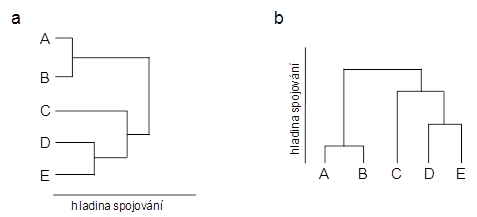
\includegraphics[width=0.515\linewidth]{Figures/hierarchial.png}
	\caption{Ukázka dendrogramu pěti objektů. Strom lze zobrazit horizontálně (a) i vertikálně (b)\cite{mat_bio}}
\end{figure}
\section{K-means shlukování}

\textbf{V centroid-bazovaném shlukování} je každý shluk reprezentován centrálním vektorem, který nemusí být členem datové sady. Když je počet shluků pevně stanoven na k, K-means shlukování poskytuje formální definici jako optimalizační problém: najít k centrálních bodů shluků a přiřadit objekty k nejbližšímu centrálnímu bodu, takže jsou minimalizovány čtvercové vzdálenosti od shluku.

Samotný optimalizační problém je znám jako NP-těžký a proto je běžným přístupem hledat pouze přibližné řešení. Zvláště dobře známou aproximativní metodou je Lloydův algoritmus, často označovaný jako "k-means algoritmus" (i když jiný algoritmus zavedl tento název). Však najde pouze lokální optimum a obvykle se spouští několikrát s různými náhodnými inicializacemi. Variace k-means často zahrnují takové optimalizace jako výběr nejlepšího z několika spuštění, ale také omezení centrálních bodů na členy datové sady (k-medoidy), volbu mediánů (k-mediánové shlukování), volbu počátečních center méně náhodně (k-means++) nebo povolení rozmazaného přiřazení k shluku (rozmazané c-means).

\begin{figure}[h]
	\centering
	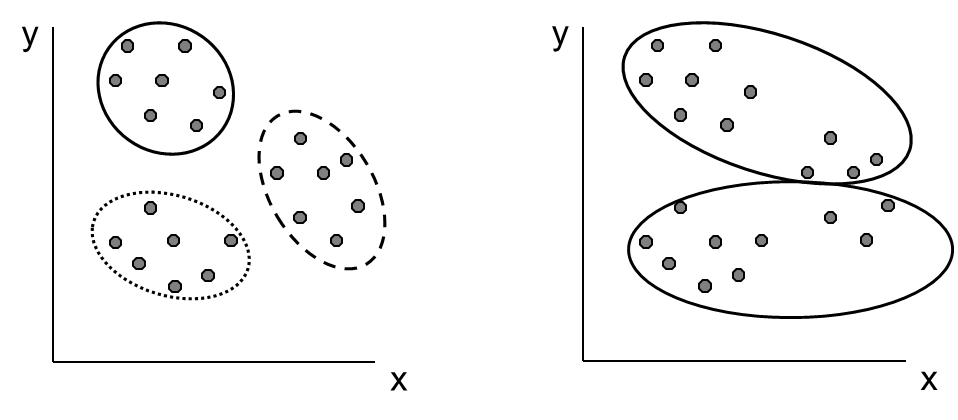
\includegraphics[width=0.515\linewidth]{Figures/kmeans.png}
	\caption{Rozdělení objektů pomocí k-means. Vlevo: k=3 (dobrá volba); vpravo: k=2 (špatná volba)\cite{mat_bio}}
\end{figure}

Většina algoritmů typu k-means vyžaduje, aby počet shluků - k - byl předem stanoven, což je považováno za jednu z největších nevýhod těchto algoritmů. Navíc algoritmy preferují shluky přibližně stejné velikosti, protože vždy přiřadí objekt k nejbližšímu centrálnímu bodu. To často vede k nesprávně ořezaným hranicím shluků (což není překvapující, protože algoritmus optimalizuje centrální body shluků, nikoli hranice shluků).

K-means algoritmus má několik výhod, např. je rychlý a efektivní pro velké množiny dat. Nicméně, pro jeho správnou aplikaci je nutné zvolit správný počet shluků k, což může být obtížné, pokud neznáme přesně strukturu dat.

Podrobnější o tom algoritmu v \textbf{Kapitole 3}.
\section{Shlukování na základě hustoty}

\textbf{Shlukování na základě hustoty (DBSCAN) }je jeden z algoritmů shlukování, který identifikuje shluky na základě hustoty v prostoru dat. Tento algoritmus umožňuje identifikovat shluky různých tvarů a velikostí, což je jedna z jeho výhod oproti jiným algoritmům shlukování.

Princip DBSCAN spočívá v nalezení oblastí s vysokou hustotou bodů, které jsou odděleny od jiných oblastí s nízkou hustotou bodů. Tato oblast s vysokou hustotou bodů představuje shluk. DBSCAN nevyžaduje určení počtu shluků předem a umožňuje identifikovat šumové body, které nejsou součástí žádného shluku.

DBSCAN má dva parametry, minimální počet bodů (MinPts) a maximální vzdálenost mezi body, které jsou stále považovány za sousední. Body v oblasti s počtem sousedních bodů větším nebo rovným MinPts jsou považovány za jádrové body a body v blízkosti jádrových bodů jsou přidány k tomuto shluku. Body, které nejsou jádrovými body ani sousedy jádrových bodů, jsou považovány za šumové body.

DBSCAN má několik výhod, například umožňuje identifikovat shluky různých tvarů a velikostí a nevyžaduje určení počtu shluků předem. Navíc dokáže identifikovat šumové body, což může být užitečné v praxi. Nicméně, DBSCAN může být náchylný k problémům v případě, kdy jsou shluky různých hustot, nebo pokud jsou shluky velmi blízko sebe, což může vést k tomu, že tyto shluky budou považovány za jeden.
\begin{figure}[h]
	\centering
	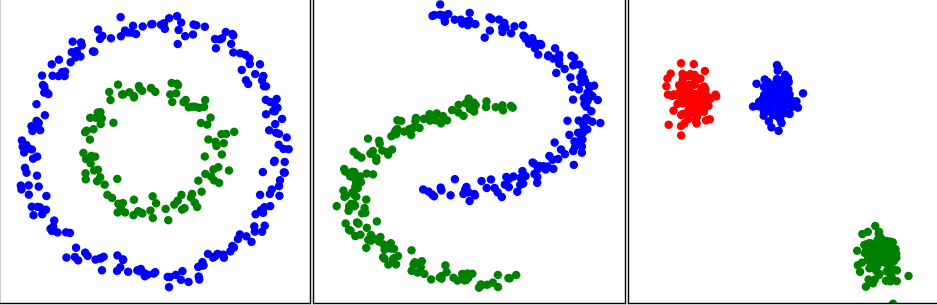
\includegraphics[width=0.515\linewidth]{Figures/dbscan.png}
	\caption{DBSCAN příklad\cite{cluster}}
\end{figure}
\chapter{K-means algoritmus}

\textbf{Postup algoritmu je následující:}
\begin{enumerate}
\item Náhodně vybereme k bodů jako počáteční středy shluků.
\item Pro každý bod určíme, do kterého shluku patří. Bod přiřadíme ke shluku s nejbližší středou.
\item Spočítáme nové středy shluků jako průměr bodů v každém shluku.
\item Vrátíme se k bodu 2 do konce interace algoritmu.
\end{enumerate}

K-means algoritmus tedy iterativně přiřazuje body ke shlukům a upravuje středy shluků, dokud nekončí počet iterace algoritmu.

\chapter{K-means experimenty}
Experimentovat s k-means budeme pomoci různych atributu aplikace. Mamé na testovaní 2 dataseta:
\begin{enumerate}
\item MallCustotomer.csv - 200 řadku
\item datesetLess.csv - 100000 řadku
\end{enumerate}

První expermient bude pomocí sekvenčního řesení algoritmu:
\begin{table}[htbp]
\centering
\label{tab:sequence}
\begin{tabular}{ |c|c|c|c| } 
 \hline
 dataset & k & pocet iterace & čas(ms) \\ 
 \hline
 MallCustotomer.csv & 5 & 10000 & 795 \\ 
 MallCustotomer.csv & 10 & 10000 & 1616 \\
 MallCustotomer.csv & 5 & 100000 & 7995 \\
 MallCustotomer.csv & 10 & 100000 & 15825 \\
 datasetLess.csv & 5 & 10000 & 40626 \\
 datasetLess.csv & 10 & 10000 & 80937 \\
 datasetLess.csv & 5 & 100000 & 408163 \\  
 \hline
\end{tabular}
\caption{Sekvenční řešení algoritmu}
\end{table}

Z toho vídíme, a to je očekované, že pokud použiváme sekvenční přistup na datasetu, který má hodně řadku tak čekaní na odpověď je nepříjemné. Proto další expreriment bude optimalizovan pomoci knihovny OpenMP.

OpenMP je knihovna pro paralelní programování v jazyce C, C++ a Fortran. Knihovna umožňuje vývojářům jednoduše vytvářet vícevláknové aplikace pro paralelní výpočty na sdílené paměti. OpenMP obsahuje sadu direktiv, které umožňují specifikovat části kódu, které mají být paralelizovány a jakým způsobem. Knihovna také poskytuje funkce pro synchronizaci vláken, jako je například kritická sekce nebo zámek.

Druhý experiment budeme provadět jen nad datasetem datasetLess.csv.
\begin{table}[htbp]
\centering
\label{tab:sequence}
\begin{tabular}{ |c|c|c|c| } 
 \hline
 dataset & k & pocet iterace & čas(ms) \\ 
 \hline
 datasetLess.csv & 5 & 10000 & 12680 \\
 datasetLess.csv & 10 & 10000 & 13182 \\
 datasetLess.csv & 5 & 100000 & 127202 \\  
 datasetLess.csv & 10 & 100000 & 128818 \\  
 \hline
\end{tabular}
\caption{OpenMP řešení algoritmu}
\end{table}

Očekaváme že zrychlení bude 2 krát, ale máme zrychlení 6 krát. Ale to je jeste přiliš dlouho. Mužeme to zlepšit pomoce knihovny OpenCL.

OpenCL (Open Computing Language) je knihovna a standard pro paralelní programování, která umožňuje vývojářům psát kód, který může běžet na různých typů výpočetních zařízeních, jako jsou CPU, GPU, FPGA a další akcelerátory. Knihovna OpenCL poskytuje rozhraní pro vytváření paralelních programů, které mohou využívat všechny dostupné výpočetní zdroje na daném zařízení.

OpenCL umožňuje programátorům specifikovat, jakým způsobem mají být paralelní výpočty prováděny, a to pomocí tzv. kernelů. Kernel je program, který se provádí na výpočetním zařízení, a je navržen tak, aby využíval co nejefektivněji jeho výpočetní kapacitu. OpenCL také obsahuje API pro komunikaci s výpočetním zařízením, pro alokaci paměti a pro spouštění kernelů.

Třetí experiment budeme provadět jen nad datasetem datasetLess.csv.
\begin{table}[htbp]
\centering
\label{tab:sequence}
\begin{tabular}{ |c|c|c|c| } 
 \hline
 dataset & k & pocet iterace & čas(ms) \\ 
 \hline
 datasetLess.csv & 5 & 10000 & 7805 \\
 datasetLess.csv & 10 & 10000 & 7942 \\
 datasetLess.csv & 5 & 100000 & 73341 \\  
 datasetLess.csv & 10 & 100000 & 74526 \\  
 \hline
\end{tabular}
\caption{OpenCL řešení algoritmu}
\end{table}

Očekaváme že zrychlení bude 2 krát, ale máme zrychlení 1.6 krát. Ale to už přijemný čas pro práce s velkymi daty.

\chapter{Zavěr}

K-means je jedním z nejčastěji používaných algoritmů pro shlukovou analýzu. Jeho implementace je relativně jednoduchá a výpočetně efektivní, což z něj dělá oblíbenou volbu pro mnoho aplikací. Nicméně, jako každý algoritmus, i k-means má své výhody a nevýhody. Mezi jeho hlavní výhody patří rychlost a skalovatelnost, zatímco nevýhody zahrnují citlivost na výběr počtu shluků, k citlivosti na vzdálenosti mezi shluky a k citlivosti na počáteční náhodnou volbu centroidů.

V seminární práci jsme se zaměřili na různé experimenty s algoritmem k-means a parallelní technologie OpenMP i OpenCL. Provedli jsme experimenty s různými datovými soubory a ukázali jsme, jak volba počtu shluků a výběr atributů mohou ovlivnit výsledky shlukování.

Celkově lze říci, že k-means je užitečný algoritmus pro mnoho aplikací, zejména pro analýzu dat a objevování skrytých struktur v datech. Nicméně, jako u každého algoritmu, je důležité důkladně zvážit jeho výhody a nevýhody a zvolit vhodný počet shluků a atributů pro danou aplikaci.

\printbibliography[title={Seznam použité literatury}]
\addcontentsline{toc}{chapter}{Seznam použité literatury}

\end{document}